% Created 2023-09-05 Tue 17:57
% Intended LaTeX compiler: pdflatex
\documentclass[9pt,twocolumn]{article}
\usepackage[utf8]{inputenc}
\usepackage[T1]{fontenc}
\usepackage{graphicx}
\usepackage{longtable}
\usepackage{wrapfig}
\usepackage{rotating}
\usepackage[normalem]{ulem}
\usepackage{amsmath}
\usepackage{amssymb}
\usepackage{capt-of}
\usepackage{hyperref}
\usepackage{algpseudocode}
\usepackage{algorithm}
\usepackage{cleveref}
\usepackage{amsthm}
\usepackage{pythonhighlight}
\usepackage{amsmath}
\usepackage{mdframed}
\BeforeBeginEnvironment{minted}{\begin{mdframed}}
\AfterEndEnvironment{minted}{\end{mdframed}}
\newtheorem{theorem}{Theorem}
\DeclareMathOperator{\diag}{diag}
\theoremstyle{definition}
\newtheorem{definition}{Definition}[section]
\author{Barak-Nadav Diker}
\date{\today}
\title{Assignment 2}
\hypersetup{
 pdfauthor={Barak-Nadav Diker},
 pdftitle={Assignment 2},
 pdfkeywords={},
 pdfsubject={},
 pdfcreator={Emacs 28.2.50 (Org mode 9.7)}, 
 pdflang={English}}
\begin{document}

\maketitle


\section*{Question 1}
\label{sec:orge35de32}

Given the following graph

\begin{center}
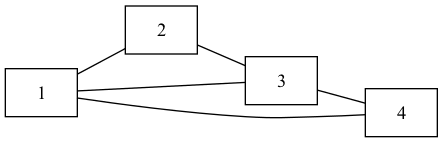
\includegraphics[width=.9\linewidth]{Question1_graph.png}
\end{center}

Calculate all walks of size 6 in the given graph

\subsection*{Answer}
\label{sec:org88b2517}
In order to do so we'll use the following theorem
\begin{theorem} [ Walks Theorem ]
If A is the adjacency matrix of a graph or digraph G with vertices \( \{v1, . . . vn\} \), then the i, j entry
of \(A^k\) is the number of walks of length k from \(v_i\) to \(v_j\)
\label{theorem-walk}
\end{theorem}

By \hyperref[theorem-walk]{Walks Theorem} we can just multiple the adjacency matrix by itself 6 times
and we'll get all the walks available from node i into node j

Since the problem specify undirected graph we'll have to sum all elements of the matrix and divide it by 2

\newpage
\begin{algorithm}
\caption{All walks of length 6 }
\begin{algorithmic}
\State \(n \gets 6 \) \Comment{6 => length of walk}
\State \( Adj  \) \Comment{adjacency matrix}
\State \( M \gets I \)
\While{ \(n \neq 0 \) }
\State \( M \gets M \times Adj \) \Comment{Matrix Multiples}
\EndWhile
\State \( sum \gets 0 \)
\While{ $a \in M $}
\State \( sum \gets sum + a \)
\EndWhile
\end{algorithmic}
\label{algo-walk}
\end{algorithm}

We will apply \textbf{algorithm} \ref{algo-walk}  for getting the number of walk of length 6

\phantomsection
\label{calculate-walks}
\begin{python}
import numpy
from numpy.linalg import matrix_power
input_array = numpy.array([[0,1,1,1],
                           [1,0,1,0],
                           [1,1,0,1],
                           [1,0,1,0]])
A_to_power6 = matrix_power(input_array, 6)
sum_var = 0
for row in A_to_power6:
    for elem in row:
        sum_var += elem
int(sum_var/2)
# output is 557
\end{python}



\section*{Question 2}
\label{sec:orge3642a3}
Consider the following quote
\begin{quote}
``Undirected Graph can be considered as directed graph''
\end{quote}
Prove it

Formally , Given an Undirected graph find a directed graph such that \(A_G = A_{G'}\)


\subsection*{Answer}
\label{sec:org35d92a6}
Given An undirected graph mark it \(G=(V,E)\) and the adjacency matrix of his as \(A_G\)

Define the directed graph \(G'=(V',E')\) where \(V'=V\) and

\[ \forall e=(v_1,v_2)\in E : e_1=(v_1,v_2) , e_2=(v_2,v_1)\in E'  \]

The adjancey matrix of the directed graph is equal to the adjancey matrix of the undirected graph

\[ A_G=A_{G'} \]


\section*{Question 3}
\label{sec:org79c8969}
Prove that given a directed graph \(G=(V,E)\) where \(V=(1,2,..,n)\) , let A be the adjacency matrix
\[ k \in \mathbb{N}\cup{\{0\}}: \forall i,j\in V : F(j,i ,k)=(A^k)_{i,j} \]
where \(F:V \times V \times \mathbb{N}\cup{\{0\}} \rightarrow \mathbb{N}\cup{\{0\}}\)
are all the walks from node j to i of length k

\subsection*{Answer}
\label{sec:orge51bc19}
We'll prove the theorem by induction
\begin{proof}
By induction

\underline{\textbf{Base Case:}}
For k = 1, \( A^k = A \), and there is a walk of length 1 between i and j
if and only if \(a_{ij} = 1\), thus the result holds.


\underline{\textbf{Step Case:}}
Assume the proposition holds for
\( k = n \) and consider the matrix \( A_{n+l} = A_nA \), By the inductive hypothesis, the
\( (i,j)^{th} \) entry of \( A_n \) counts the number of walks of length n between vertices i
and j. Now, the number of walks of length n + 1 between i and j equals the
number of walks of length n from vertex i to each vertex v that is adjacent to j.
But this is the \( (i,j)^{th} \) entry of \( A^nA = A^{n+1} \) the non-zero entries of the column
of A corresponding to v are precisely the first neighbours of v. Thus the result
follows by induction on n
\end{proof}

\section*{Question 4}
\label{sec:orgd02a53c}
Find the number of possible walks of length 8 from 1 to 4 by the following undirected graph

\begin{center}
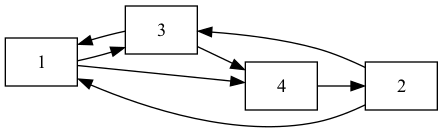
\includegraphics[width=.9\linewidth]{Question4_graph.png}
\end{center}
\subsection*{Answer}
\label{sec:org7d8fd95}
We'll Write the adjancey matrix and calculate the \(A^8\)

To do so we'll use the same code

\phantomsection
\label{calculate-question4-walks}
\begin{python}
import numpy
from numpy.linalg import matrix_power
input_array = numpy.array([[0,1,1,0],
                           [0,0,0,1],
                           [1,1,0,0],
                           [1,0,1,0]])
A_to_power6 = matrix_power(input_array, 8)
A_to_power6[3][0]
# output is 23
\end{python}

To Calculate the Matrix by power of 8 we will use eigen values \(\det(A-\lambda I_n) = 0\) lets apply the calculation
\[
\det(A-\lambda I_n) =\begin{vmatrix}
 -\lambda & 1 & 1 & 0 \\[0pt]
 0 & -\lambda & 0 & 1 \\[0pt]
 1 & 1 & -\lambda & 0 \\[0pt]
 1 & 0 & 1 & -\lambda \\[0pt]
\end{vmatrix}= 0
\]

In order to find eigen value will python code
\phantomsection
\label{calculate-question4-walks-python}
\begin{python}
import numpy as np
from numpy.linalg import eig
input_array = np.array([[0,1,1,0],
                           [0,0,0,1],
                           [1,1,0,0],
                           [1,0,1,0]])
w,v=eig(input_array)

w # The vector of eigen values
# w = | 1.69 | -1 | +0.j | -0.347-1.028j |

\end{python}

And finally we do
\[
p^{-1}A^8p =\begin{pmatrix}
 \lambda^8_1 & 0 & 0 & 0 \\[0pt]
 0 & \lambda^8_2 & 0 & 0 \\[0pt]
 0 & 0 & \lambda^8_3 & 0 \\[0pt]
 0 & 0 & 0 & \lambda^8_4 \\[0pt]
\end{pmatrix}
\]


and change basis to get

\[
A^8 =\begin{pmatrix}
 19 & 23 & 18 & 13 \\[0pt]
 13 & 14 & 13 & 10 \\[0pt]
 18 & 23 & 19 & 13 \\[0pt]
 23 & 26 & 23 & 14 \\[0pt]
\end{pmatrix}
\]
\section*{Question 5}
\label{sec:org749cd62}
Prove that the probablity to pass from vertex j to vertex i is given by
the matrix \(\tilde{A_G} = A_G*D^{-1}_G\)
where the matrix \(D_G\) is define to be

\[
D_G =\begin{pmatrix}
 \deg(1) & 0 & ... & 0 \\[0pt]
 0 & \deg(2) & ... & 0 \\[0pt]
 0 & 0 & ... & 0 \\[0pt]
 0 & 0 & ... & \deg(n) \\[0pt]
\end{pmatrix}
\]



careful \(\tilde{A_G}\) might not be symmetric

\subsection*{Answer}
\label{sec:org5f3182e}

\begin{proof}
Since G is undirected graph and the probablity to travel from j to i is even distributed ,
the probability matrix is to divide the matrix \(A_G\) column j by \( \deg(j) \) for each \( j \in \mathbb{N}\cap [1,n] \)
or more formally
\[
\forall j \in \mathbb{N}\cap [1,n] \,, ( \hat{A_G} )_{i,j} := \frac{(A_G)_{i,j}}{\deg(j)}
\]

But Happily this is exactly equivalent to simply multiply the following matrix
\[
\tilde{A_G} = A_G*D^{-1}_G
\]
i.e
\[
\tilde{A_G} = \hat{A_G}
\]
Which is what we want it to be
\end{proof}


\section*{Question 6}
\label{sec:org4671f85}
let \(p^{(0)}\in \mathbb{R}\) be the initial probability distribution of the graph

let \(p^{(n)} \in \mathbb{R}\) be the distribution of the graph after n walks

prove that
\[
p^{(n)} = \tilde{A_G^n} * p^{( 0 )}
\]



\subsection*{Answer}
\label{sec:org4a829e5}
\begin{proof}
Given a vertex j and vertex i we first want to find all possible walks from j to i with length n ,

We have already proven that the number of possible walks are \( ( A_G^n )_{i,j} \)

In order to get the required probability we need to find the sum of all walks from j to any vertex i.e
\[
\sigma _j = \sum _{i\in V} ( A_G )_{i,j}^{n}
\]

\[
( Prob )_{i,j} = \frac{(A_G^n)_{i,j}} { \sigma _j }
\]

Ultimately , I have proven that the probability of walking n walks from vertex j to i is simply
\( \tilde{A}^n \)

\end{proof}

Note that we are not yet done we still have to prove that
\[
p^{(n)} = \tilde{A}^n * p^{(0)}
\]

To skip to that click \hyperref[final-prove]{final}

Another proof is by induction

\begin{proof}
\( \tilde{A}^{m+1} = \tilde{A} * \tilde{A}^{m}\)

\underline{\textbf{Base Case:}}
for n=0 we have \(\tilde{A} = \tilde{A}\)

\underline{\textbf{Step Case:}}
Given that the claim is true for \(n\in \mathbb{N}\) we will prove it for \(n+1\) ,
more specificly given j and i we are searching for the probablity of going from j to i  after \(n+1\) walks

Since by assumption we already know the probabilty of walking n long from j to any \(v\in V\)
 which is \( (A_G^n)_{v,j} \) and also
we know the probablity of getting from any vertex v into vertex i which is \( ( A_G )_{i,v}  \)

The probabilty of getting from j to i after n+1 walks is by conditional probabilty

\[ Prob^{(n+1)} =  \sum_{v\in V} (A_G)_{i,v}*(A_G^n)_{v,j}\]
since
\[
P(B) = \sum_{i} P(B|A_i) \,, \sum _{i} P(A_i) = 1
\]

This equation is nothing but \( \tilde{A}^{m+1} = \tilde{A} * \tilde{A}^{m}\)
\end{proof}

Now Given a vertices \(i \in V\) by the complete probability theorem the probability of getting into vertex i is
\[ p^{(n)}_i = \sum_{v \in V} \tilde{A}_{i,v}*p^{(0)}_v \]
But this equation is nothing but what we needed to prove which is
\begin{equation}
\label{final-prove}
p^{(n)} = \tilde{A}^n * p^{(0)}
\end{equation}



\section*{Question 7}
\label{sec:org56f79a5}
Prove that \(\tilde{A}\) is diagolizable over \(\mathbb{R}\)

\subsection*{Answer}
\label{sec:org9250fec}
We will use the spectral theory for the prove

\href{https://en.wikipedia.org/wiki/Spectral\_theory}{Spectral Theory}

\begin{math}
\underline{\textbf{Reminder:}}
\end{math}
Please Note that \(\tilde{A}=A_G*D^{-1}\)

By assumption , we know A is a symmetric matrix ,

lets mark the matrix
\[ Q\in \mathbb{M}_n(\mathbb{R}) : Q := \diag(\sqrt{ \deg(v_1) },\dots , \sqrt{ \deg(v_n)) } \]

Observe the following logic:

\[
Q^{-1}*\tilde{A}*Q=Q^{-1}*A*D^{-1}*Q=Q^{-1}*A*Q^{-1}
\]
where \(A=A^{t}\)

\begin{align*}
(Q^{-1}*A*Q^{-1})^{t}&=(A*Q^{-1})^t*(Q^{-1})^t= \\
                    &=(Q^{-1})^t*A^t*(Q^{-1})^t \\
                    &=(Q^{-1})^t*A*(Q^{-1})^t \\
                    &=Q^{-1}*A*Q^{-1}
\end{align*}
By this equation we can infer that the matrix

\(Q^{-1}*\tilde{A}*Q\) is
a symmetric matrix which means that we can use on it the spectral theory

\[
\exists P\in \mathbb{M}_n(\mathbb{R}) : P^{-1}*(Q^{-1}*\tilde{A}*Q)*P = \diag(\lambda _1 , \lambda _2 , \dots , \lambda _n)
\]
\[
=(QP)^{-1}\tilde{A}QP
\]

So I have found a matrix QP which diagolize the matrix \(\tilde{A}\)






\section*{Question 8}
\label{sec:org661e71c}

let \(\lambda\) be an eigen value of \(\tilde{A}\) proof that
\(\lambda\in [-1,1]\)

\subsection*{Answer}
\label{sec:org104feee}
I'll prove it by contradiction , on the matrix \(\tilde{A}^t\), let \(\lambda\) be eigen value of \(\tilde{A}\)
\[\exists v\in V : \tilde{A}v=\lambda v\]
for some \(\lambda > 1\)

Since the row of the matrix \(\tilde{A}^t\) sums to 1 , each element of \(\tilde{A}^tx\) is an
\href{https://en.wikipedia.org/wiki/Convex\_combination}{convex combination} of the components of x , which can't be greater than a \(x_{max}\) where \(x_{max}\) is the maxium
element of the vector x .

Let's see it formally

\[
x_{max} := \max_{j\in\mathbb{N}\cap [1,n]}{|x_j|}
\]
\[
\alpha := \tilde{A}^t
\]
\[
\forall \mathbb{N}\cap [1,n] \sum_{j=1}^{n} \alpha_{ij} = 1
\]
\begin{align*}
\forall x\in \mathbb{R}^{n} \,, \forall i\in\mathbb{N}\cap [1,n]  \,, \sum_{j=1}^n\alpha _{ij} x_{j}  &\leq\sum_{j=1}^n \alpha_{ij}x_{max}= \\
                                                                    &=x_{max} \sum_{j=1}^{n} \alpha_{ij} = x_{max}
\end{align*}
In conclusion

\begin{equation}
\label{label-equ1}
(\tilde{A}^t x)_{max} \leq x_{max}
\end{equation}

On the other hand , At least one element of \(\lambda x\) is greater than \(x_{max}\) , which proves that
\(\lambda > 1\) is impossible

Or , more precisely , let \(\lambda > 1\) be an eigen value of the matrix
\(\tilde{A}^t\) and let \(v_{\lambda}\) be the normalized eigen vector of
eigen value \(\lambda\) then

\begin{equation}
\label{label-equ2}
(v_{\lambda})_{max} <
\lambda (v_{\lambda})_{max} =
( \lambda v_{\lambda} )_{max} =
( \tilde{A}^t v_{\lambda} )_{max}
\end{equation}

By equation \ref{label-equ1} we can select \(x:=v_{\lambda}\) and we'll have
\((\tilde{A}^t v_{\lambda})_{max} \leq (v_{\lambda})_{max}\) which contradict equation \ref{label-equ2}





\section*{Introduction}
\label{sec:org7ade61d}

\section*{{\bfseries\sffamily TODO} Simple pseudo code\hfill{}\textsc{ATTACH}}
\label{sec:orgd8d4fe5}
\begin{itemize}
\item Note taken on \textit{[2023-07-05 Wed 14:42] } \\[0pt]
Hello World !!!
\item Note taken on \textit{[2023-07-05 Wed 14:37] } \\[0pt]
BARAKKKK
\item Note taken on \textit{[2023-07-05 Wed 14:36] } \\[0pt]
Hello World !!
\item Note taken on \textit{[2023-07-05 Wed 14:36] } \\[0pt]
Barak the King
\end{itemize}
Hello World
\begin{displaymath}
\lambda *6
\end{displaymath}

0:00:23
0:01:17
0:01:20
0:01:22
\href{https://orgmode.org/org.html\#Tables-in-LaTeX-export}{The Org Manual}
0:01:22

0:01:22
0:01:22
0:01:22
0:01:22 0:01:22 0:01:22 0:01:22 0:01:22
0:00:03 0:00:05 0:00:07 0:00:08 0:00:09 0:00:09 0:00:00 0:00:03 0:00:04
0:00:06 0:00:07 0:00:00 0:00:00 0:00:02 0:00:03 0:00:02 0:00:03
\section*{{\bfseries\sffamily IDEA} }
\label{sec:orgf389a63}
\section*{{\bfseries\sffamily KILL} }
\label{sec:org609a9d6}
\section*{{\bfseries\sffamily IDEA} }
\label{sec:org8875032}
\end{document}